% 独自のコマンド

% ■ アブストラクト
%  \begin{jabstract} 〜 \end{jabstract}  :日本語のアブストラクト
%  \begin{eabstract} 〜 \end{eabstract}  :英語のアブストラクト

% ■ 謝辞
%  \begin{acknowledgment} 〜 \end{acknowledgment}

\newif\ifjapanese

\japanesetrue  % 論文全体を日本語で書く(英語で書くならコメントアウト)

\ifjapanese
  %\documentclass[a4j,twoside,openright,11pt]{jreport} % 両面印刷の場合.余白を綴じ側に作って右起こし.
  \documentclass[a4j,11pt]{jreport}                  % 片面印刷の場合.
  \renewcommand{\bibname}{参考文献}
  \newcommand{\acknowledgmentname}{謝辞}
\else
  \documentclass[a4paper,11pt]{report}
  \newcommand{\acknowledgmentname}{Acknowledgment}
\fi
\usepackage[dvipdfmx]{graphicx}
\usepackage{thesis}
\usepackage{ascmac}
\usepackage{graphicx}
\usepackage{multirow}
\usepackage{url}
\usepackage{latexsym}
\usepackage{here}
\usepackage{listings,jlisting}

\lstset{%
  language={C},
  basicstyle={\small\ttfamily\footnotesize},%
  breaklines=true,%
  identifierstyle={\small},%
  commentstyle={\small\itshape},%
  keywordstyle={\small\bfseries},%
  ndkeywordstyle={\small},%
  stringstyle={\small\ttfamily},
  frame={tb},
  breaklines=true,
  columns=[l]{fullflexible},%
  numbers=left,%
  xrightmargin=0zw,%
  xleftmargin=3zw,%
  numberstyle={\scriptsize},%
  stepnumber=1,
  numbersep=1zw,%
  lineskip=-0.5ex%
}
\bibliographystyle{jplain}

%\bindermode  % ファイル綴じ用余白設定

% 日本語情報(必要なら)
\jclass  {卒業論文}                             % 論文種別
\jtitle  {情報の鮮度を視覚化する検索システムの研究} % タイトル.改行する場合は\\を入れる
\juniv   {慶應義塾大学}                   % 大学名
\jfaculty{環境情報学部}                 % 学部,学科
\jauthor {二塚 康平}                            % 著者
\jhyear  {3}                                   % 令和○年度
\jsyear  {2021}                                 % 西暦○年度
\jkeyword{情報検索,ブラウザ,情報視覚化,情報の鮮度}       % 論文のキーワード
\jproject{増井俊之研究会} % プロジェクト名
\jdate   {2021年1月}

\begin{document}

\ifjapanese
  \jmaketitle    % 表紙(日本語)
\else
  \emaketitle    % 表紙(英語)
\fi

% ■ アブストラクトの出力 ■
%	◆書式:
%		begin{jabstract}〜end{jabstract}	:日本語のアブストラクト
%		begin{eabstract}〜end{eabstract}	:英語のアブストラクト
%		※ 不要ならばコマンドごと消せば出力されない。



% 日本語のアブストラクト
\begin{jabstract}

本論文では、Web 上の情報検索における検索結果一覧画面でそれぞれの情報の鮮度が一目で分かるシステムを提案する。

一般的な Web ブラウザでは、検索した情報がいつ公開されたかに応じて表示に差を設けることはしていないが、情報の取捨選択において情報の鮮度は重要な要素の一つである。

そこで、情報の表示に実世界における情報媒体が劣化していくメタファを適用することで、ユーザが検索した情報の鮮度をより直感的に認識することができる。

\end{jabstract}
  % アブストラクト.要独自コマンド,include先参照のこと

\tableofcontents  % 目次
\listoffigures    % 図目次
% \listoftables    % 表目次

\pagenumbering{arabic}

\chapter{序論}
\label{chap:introduction}

本章では,本研究の背景と本論文の構成について述べる.

\newpage

\section{背景}

Webブラウザ上での情報検索が近年広く利用されている.

我々は普段情報検索を行う際,古い情報よりも新しい情報を求めていることが多いと考えられる.つまり古い情報よりも新しい情報の方が価値が高いのである.

しかし,Web 検索の結果一覧画面における各情報は,実世界に存在する紙やインクのように時間経過による外見的な劣化がないため,情報の鮮度を直感的に判断するのは難しい.

\begin{figure}[htbp]
  \begin{minipage}{0.5\hsize}
    \begin{center}
      \fbox{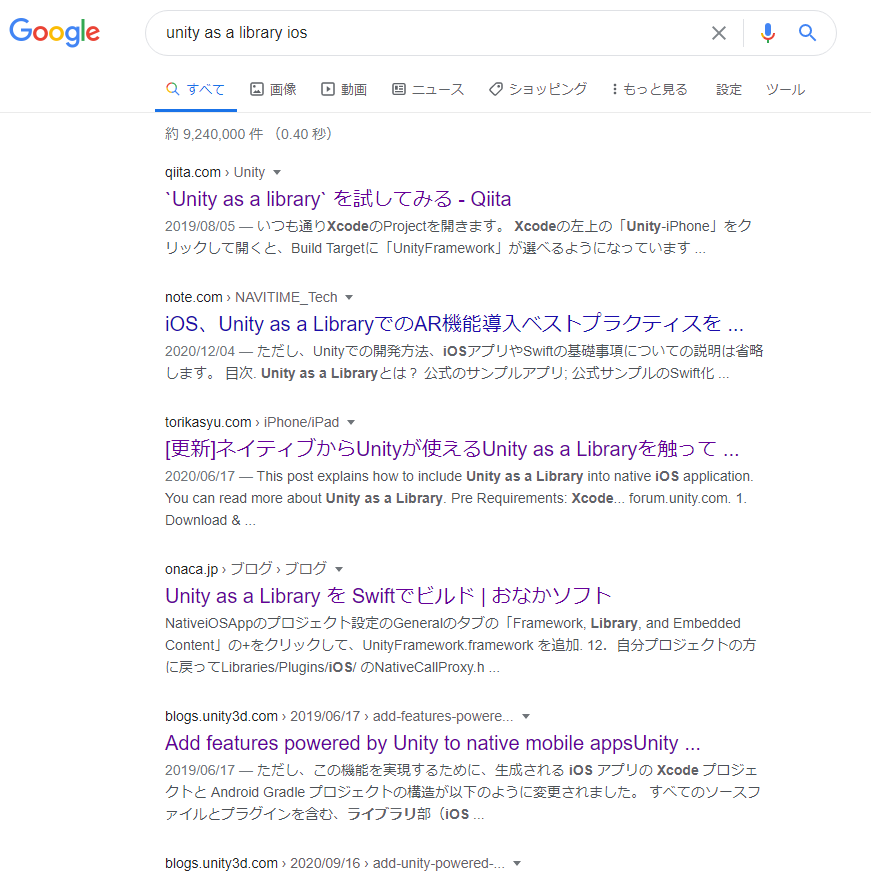
\includegraphics[width=60mm]{images/search-google.png}}
    \end{center}
    \caption{Google の検索結果一覧画面}
  \end{minipage}
  \begin{minipage}{0.5\hsize}
    \begin{center}
      \fbox{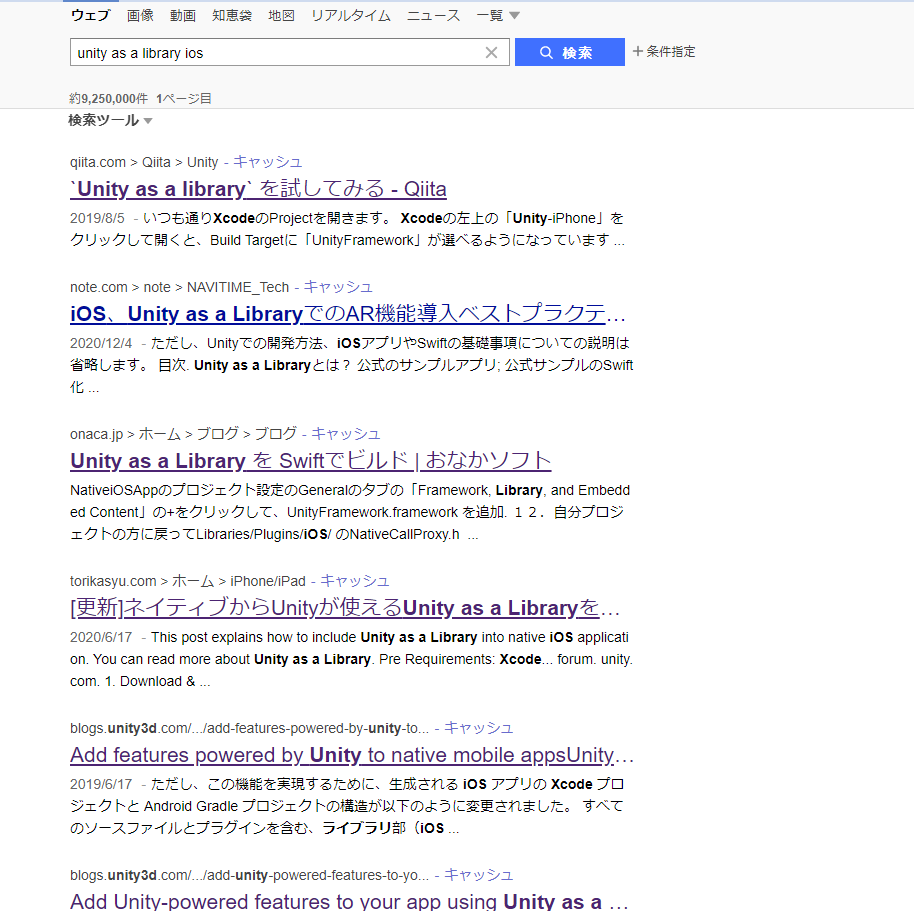
\includegraphics[width=60mm]{images/search-yahoo.png}}
    \end{center}
    \caption{Yahoo! の検索結果一覧画面}
  \end{minipage}
\end{figure}
\begin{figure}[htbp]
  \begin{minipage}{0.5\hsize}
    \begin{center}
      \fbox{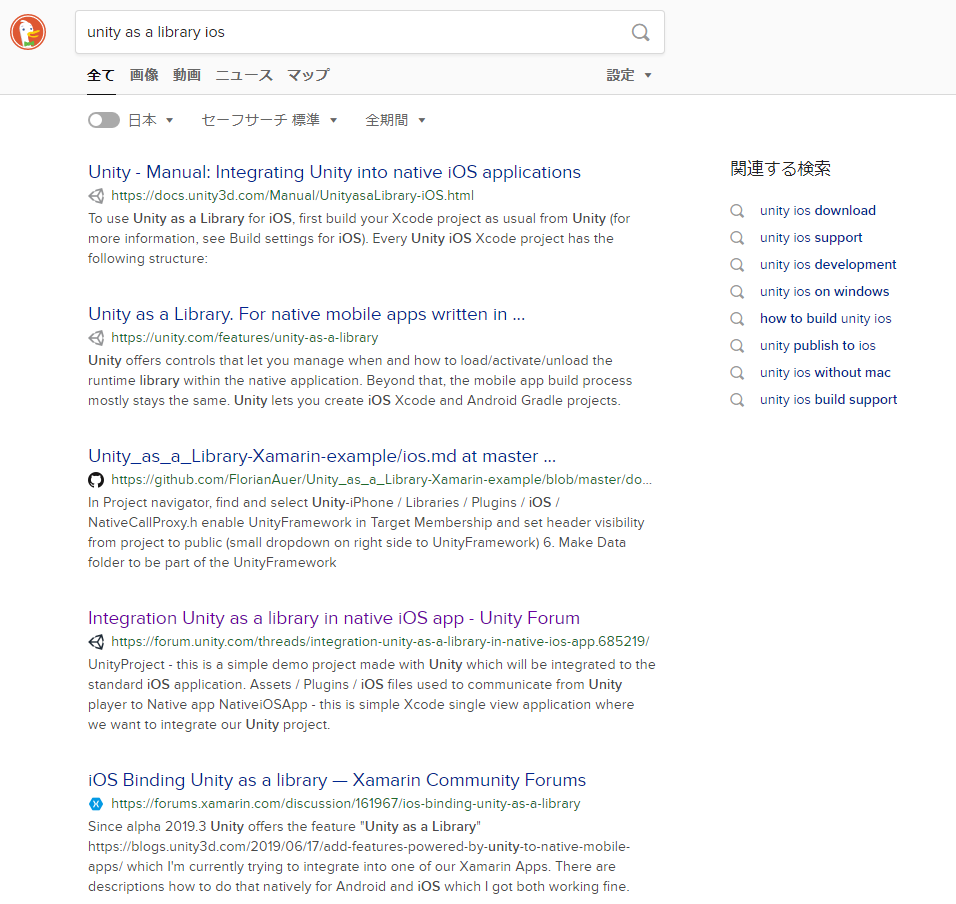
\includegraphics[width=60mm]{images/search-ddg.png}}
    \end{center}
    \caption{DuckDuckGo の検索結果一覧画面}
  \end{minipage}
  \begin{minipage}{0.5\hsize}
    \begin{center}
      \fbox{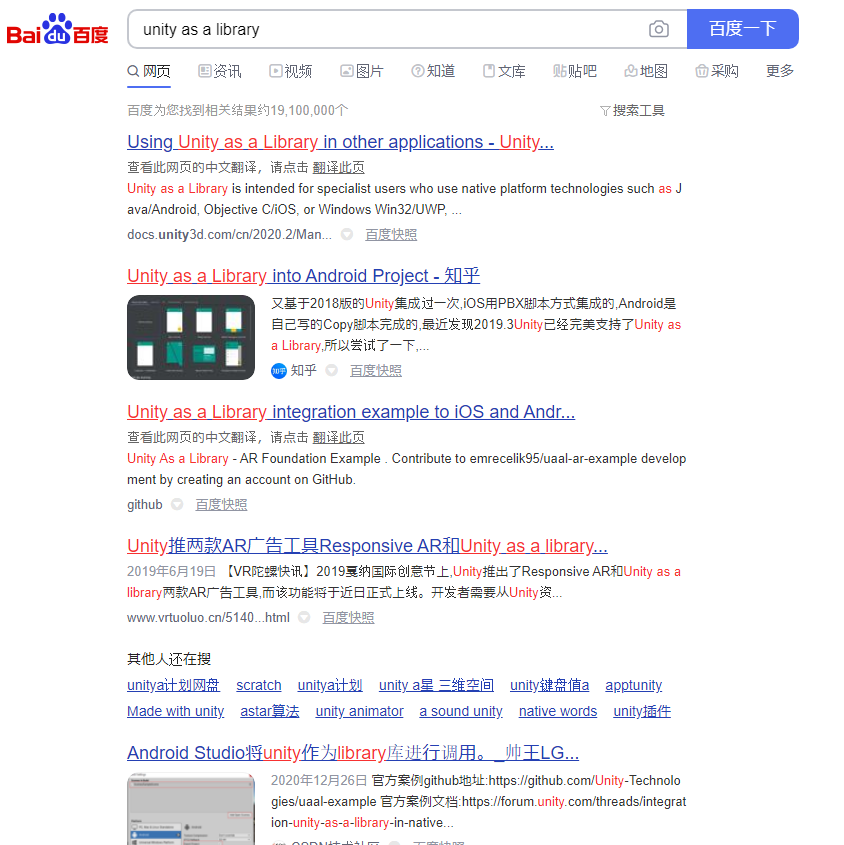
\includegraphics[width=60mm]{images/search-baidu.png}}
    \end{center}
    \caption{Baidu の検索結果一覧画面}
  \end{minipage}
\end{figure}

そこで,本来外見的な劣化のない各情報に,時間経過による表示の変化を与える.これにより情報の鮮度を直感的に認識できるようになり,Web 検索による情報収集を効率的に行えると考えた.

% こういった Web 検索結果一覧画面での情報の視覚化に関して,松下らは「ネット上の情報を可視化する技術」\cite{tecvisinfo}で,

% \begin{quote}
%   Web の規模が膨大になるにつれ,ランキングの精度がますます大きな問題となるが,精度向上にも限界があるため,情報可視化システムにかかる期待も今後大きくなると予想される.
% \end{quote}

% と述べている.

% また,ユーザが検索結果から最初の選択をするまでにかける時間が平均5.7秒だという調査\cite{pinball}があり,この短い時間でユーザに情報の鮮度を認識させなければならない.

リンク先のページの鮮度に応じてリンクの表現を変化させる「廃れるリンク」\cite{dyinglink}のようなシステムも存在するが,リンクのみへの適用であるため鮮度の表現方法に改善の余地があると考えた.

\section{本研究の目的}

本研究の目的は,ユーザがより直感的に情報の鮮度を認識できるように,ブラウザにおける検索結果一覧画面の表示を拡張することである.

\section{本文書の構成}

第\ref{chap:introduction}章では本研究における背景と目的について述べる.

第\ref{chap:verification}章では実際に視覚化システムを開発する前に様々な視覚化の方法を試し評価する.

第\ref{chap:implementation}章で開発したシステムの実装に関して述べ,第\ref{chap:discussion}章では実際に利用して得られた評価や今後の展望について述べる.

第\ref{chap:survey}章では本研究と関連のある研究事例を紹介している.第\ref{chap:conclusion}章では本研究を総括して結論を述べる.
  % 本文1
\chapter{鮮度の表現方法の検証}
\label{chap:verification}

本章では、情報の鮮度の視覚化について様々な視覚化の方法を試し、それぞれ考察していく。

以下で検証する全ての項目に関して図\ref{fig:ver-base}を利用する。

\begin{figure}[htbp]
  \begin{center}
    \fbox{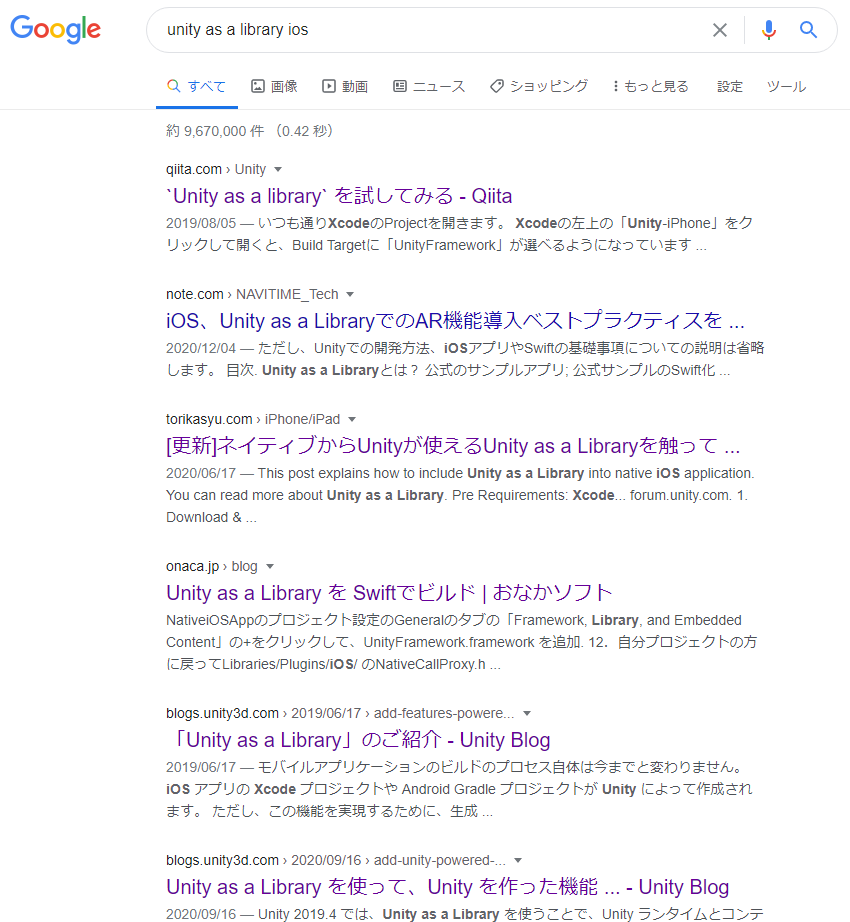
\includegraphics[width=60mm]{images/base.png}}
  \end{center}
  \caption{視覚化前の検索結果一覧}
  \label{fig:ver-base}
\end{figure}


\section{テクスチャによる変化}
\label{sec:ver-texture}

テクスチャを適用することで鮮度を視覚化する方法を検証する。

\subsection{紙の経年劣化}
\label{subsec:ver-tex-sheet}

実世界に存在する記録媒体で劣化するものを考えたときに最初に思い浮かんだのが紙である。

紙は時間が経つと黄ばみやシミができる。そういった変化を参考に、情報の鮮度を視覚化した。

\begin{figure}[htbp]
  \begin{minipage}{0.5\hsize}
    \begin{center}
      \fbox{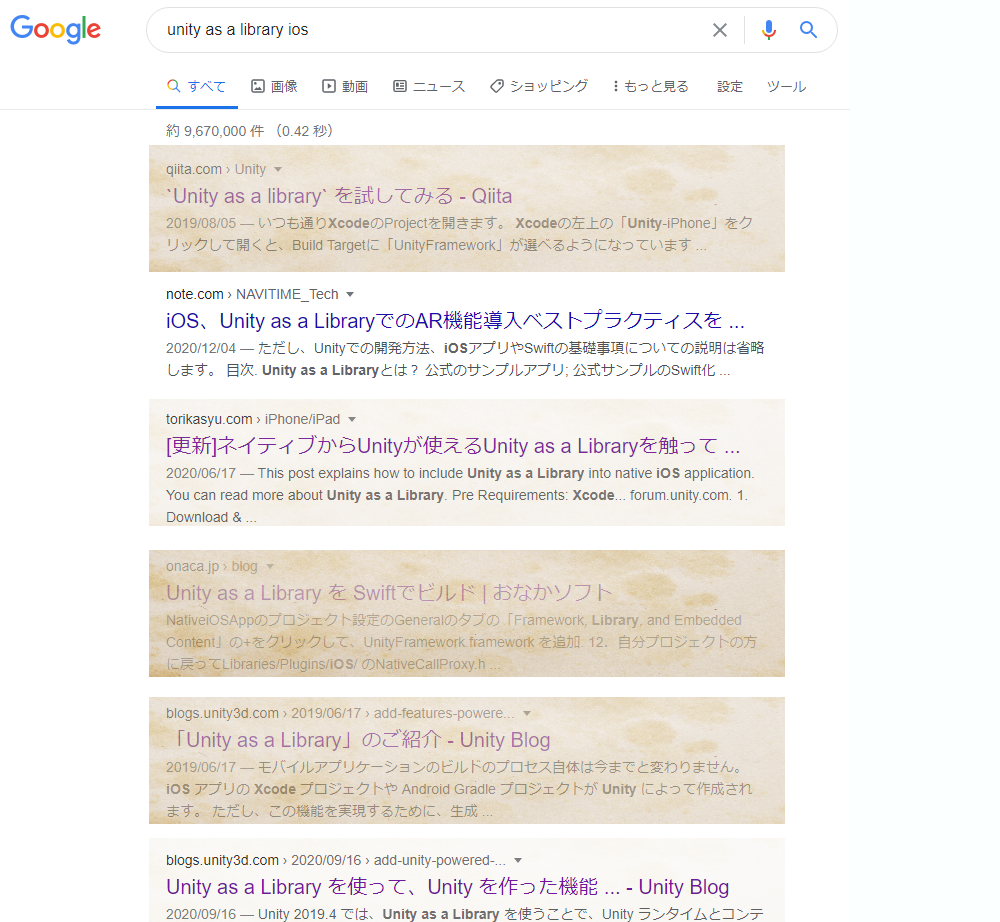
\includegraphics[width=60mm]{images/sheet-degradation1.png}}
    \end{center}
    \caption{紙の経年劣化をイメージした視覚化1}
    \label{fig:ver-sheet1}
  \end{minipage}
  \begin{minipage}{0.5\hsize}
    \begin{center}
      \fbox{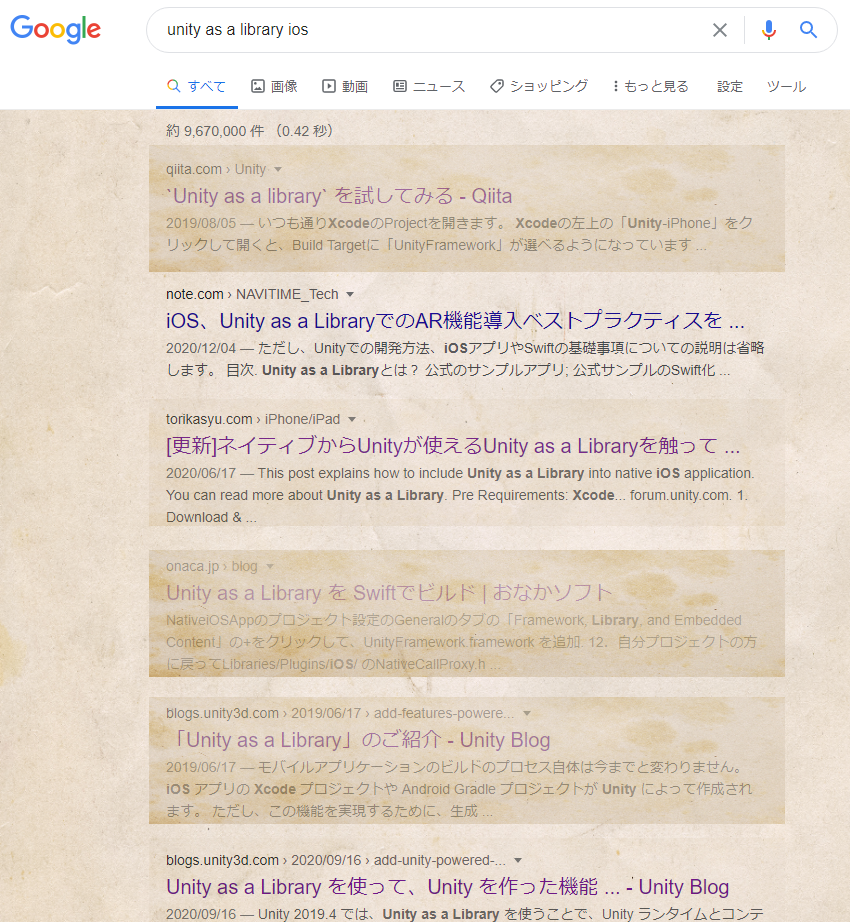
\includegraphics[width=60mm]{images/sheet-degradation2.png}}
    \end{center}
    \caption{紙の経年劣化をイメージした視覚化2}
    \label{fig:ver-sheet2}
  \end{minipage}
\end{figure}

各検索結果ごとに公開日を参考に、劣化した紙のテクスチャを適用したのが図\ref{fig:ver-sheet1}である。

さらに、全体に紙のテクスチャを適用することで劣化した紙のテクスチャが背景になじむように調整したのが図\ref{fig:ver-sheet2}である。

紙の劣化を参考にしているためか、古いということが分かりやすい。家や図書館などで古くなった本を見た経験がある人ならば、紙の時間経過による劣化を連想しやすいのではないだろうか。

図\ref{fig:ver-sheet1}に比べて、図\ref{fig:ver-sheet2}の方が背景に紙のテクスチャを設定しているため劣化した紙のテクスチャに違和感が少ない。

\subsection{金属のさび}
\label{subsec:ver-tex-russet}

実世界に存在するモノで紙以外に外見的な劣化の参考になるものを考えたとき、次に浮かんだのは金属である。

金属は雨風にさらされることでさびが発生するため、時間経過による劣化が簡単に見て取れる。これを参考に視覚化を行った。

\begin{figure}[htbp]
  \begin{minipage}{0.5\hsize}
    \begin{center}
      \fbox{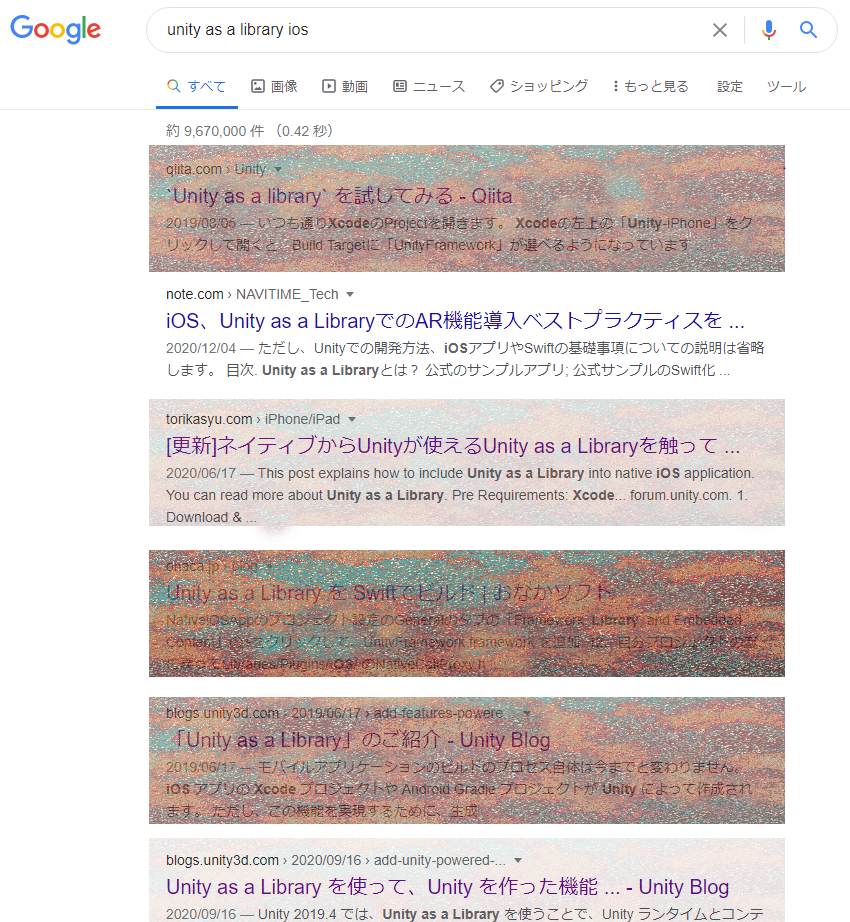
\includegraphics[width=60mm]{images/iron-russet1.png}}
    \end{center}
    \caption{金属のさびをイメージした視覚化1}
    \label{fig:ver-russet1}
  \end{minipage}
  \begin{minipage}{0.5\hsize}
    \begin{center}
      \fbox{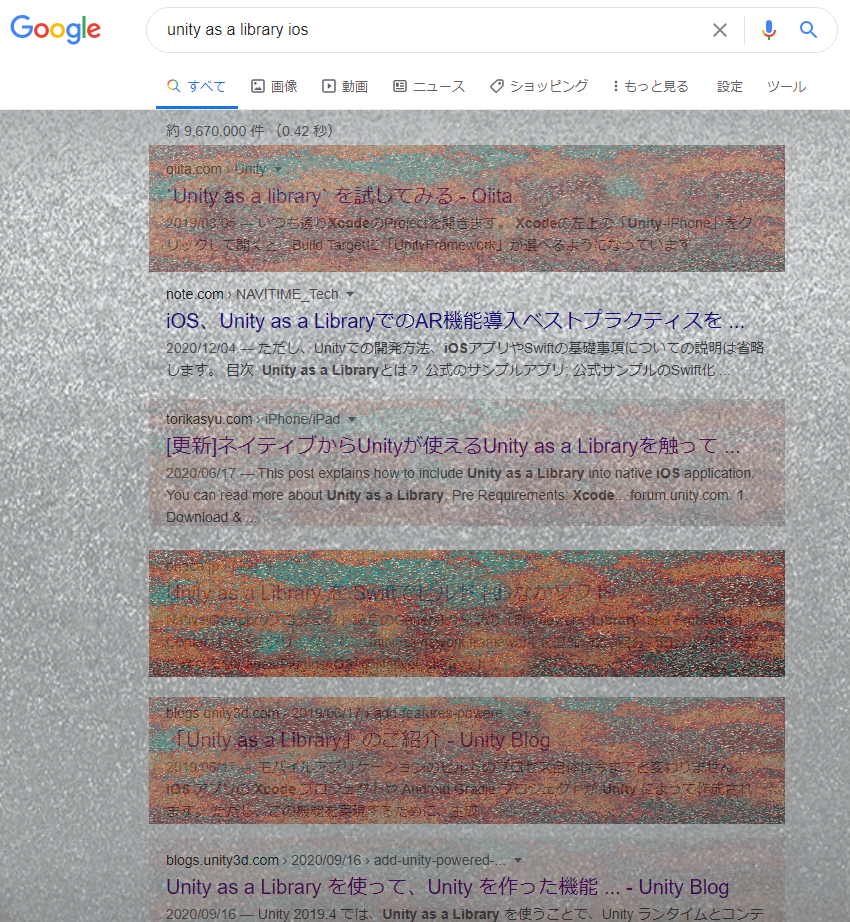
\includegraphics[width=60mm]{images/iron-russet2.png}}
    \end{center}
    \caption{金属のさびをイメージした視覚化2}
    \label{fig:ver-russet2}
  \end{minipage}
\end{figure}

\ref{subsec:ver-tex-sheet}の方法と同様に、錆びた金属のテクスチャを適用したのが図\ref{fig:ver-russet1}である。

また、背景に錆びていない金属のテクスチャを適用したのが図\ref{fig:ver-russet2}である。

\ref{subsec:ver-tex-sheet}と比べて古い情報が強調されているが、背景に金属のテクスチャを適用してもぬぐい切れない不自然さがある。

文字が記録されている媒体として金属があまり適していないことが原因と推測される。

\section{色による変化}
\label{sec:ver-color}

背景色や文字色を変更することで鮮度を視覚化する方法を検証する。

\subsection{背景の色褪せ}
\label{subsec:ver-col-cor}

実世界のモノが腐食するイメージを参考に、背景の色褪せによって情報の鮮度を視覚化した。

\begin{figure}[htbp]
  \begin{minipage}{0.5\hsize}
    \begin{center}
      \fbox{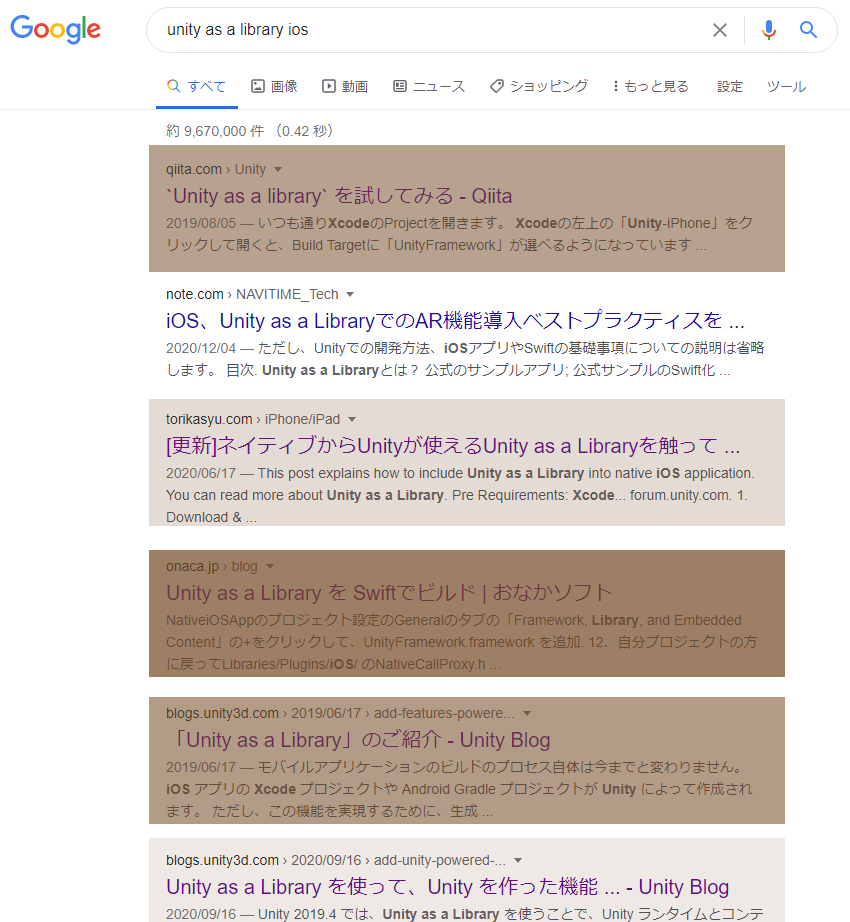
\includegraphics[width=60mm]{images/corrosion1.png}}
    \end{center}
    \caption{腐食をイメージした視覚化1}
    \label{fig:ver-corrosion1}
  \end{minipage}
  \begin{minipage}{0.5\hsize}
    \begin{center}
      \fbox{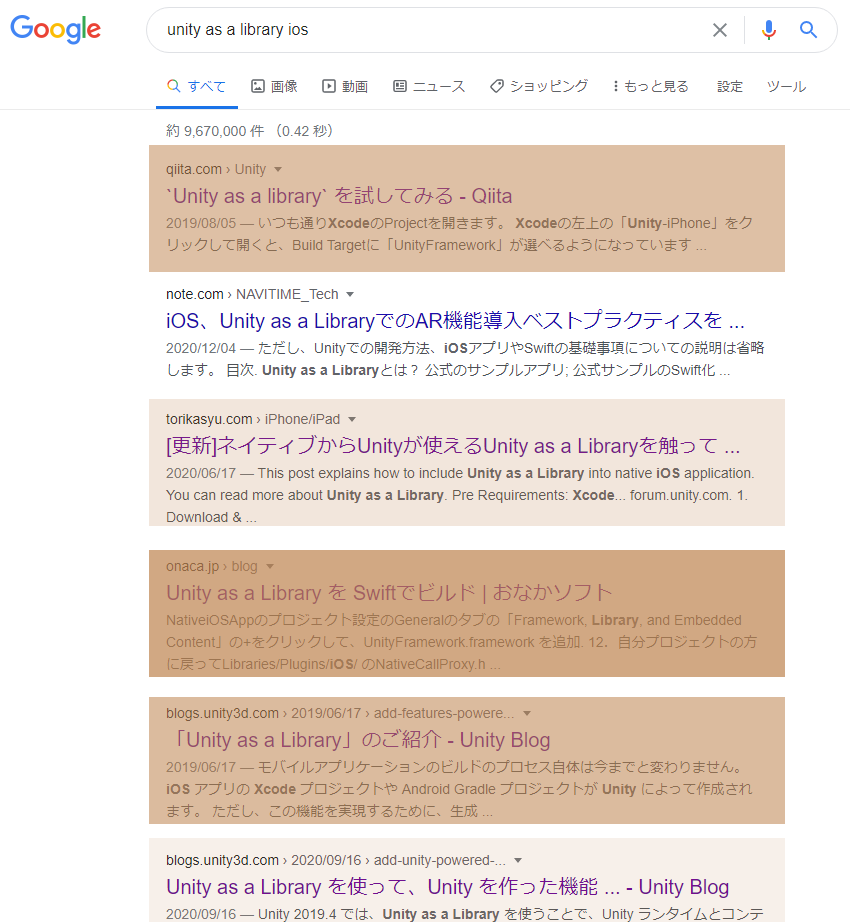
\includegraphics[width=60mm]{images/corrosion2.png}}
    \end{center}
    \caption{腐食をイメージした視覚化2}
    \label{fig:ver-corrosion2}
  \end{minipage}
\end{figure}

腐食を参考にしたため暗い茶色(図\ref{fig:ver-corrosion1})や赤茶色(図\ref{fig:ver-corrosion2})の中で鮮度ごとに色が変化するように、視覚化を適用している。

コンセプトとしては\ref{sec:ver-texture}で検証した二つと近いが、こちらの方がシンプルな分、元の白い背景に対して不自然さがないが、鮮度を示すものということが認識しにくい。

色の選定部分においては議論の余地があると考えられる。

\subsection{インクの劣化}
\label{subsec:ver-col-ink}

紙に書いた文字のインクが時間経過によって劣化していくのを参考に、情報の鮮度を視覚化した。

\begin{figure}[htbp]
  \begin{minipage}{0.5\hsize}
    \begin{center}
      \fbox{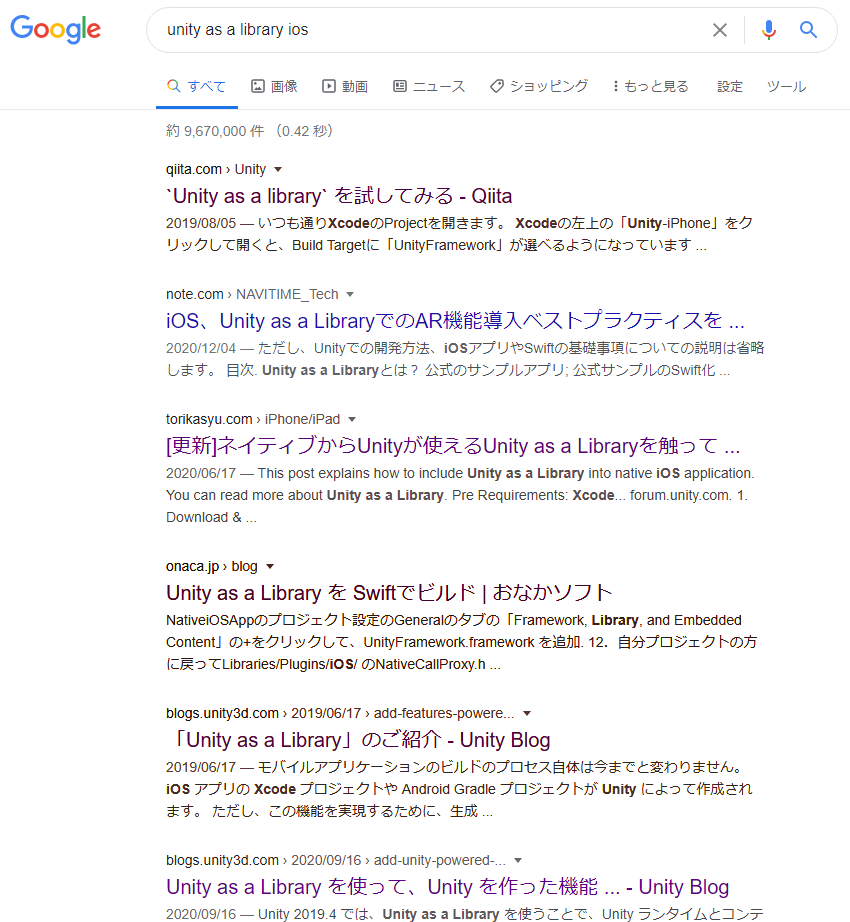
\includegraphics[width=60mm]{images/ink1.png}}
    \end{center}
    \caption{インクの劣化をイメージした視覚化1}
    \label{fig:ver-ink1}
  \end{minipage}
  \begin{minipage}{0.5\hsize}
    \begin{center}
      \fbox{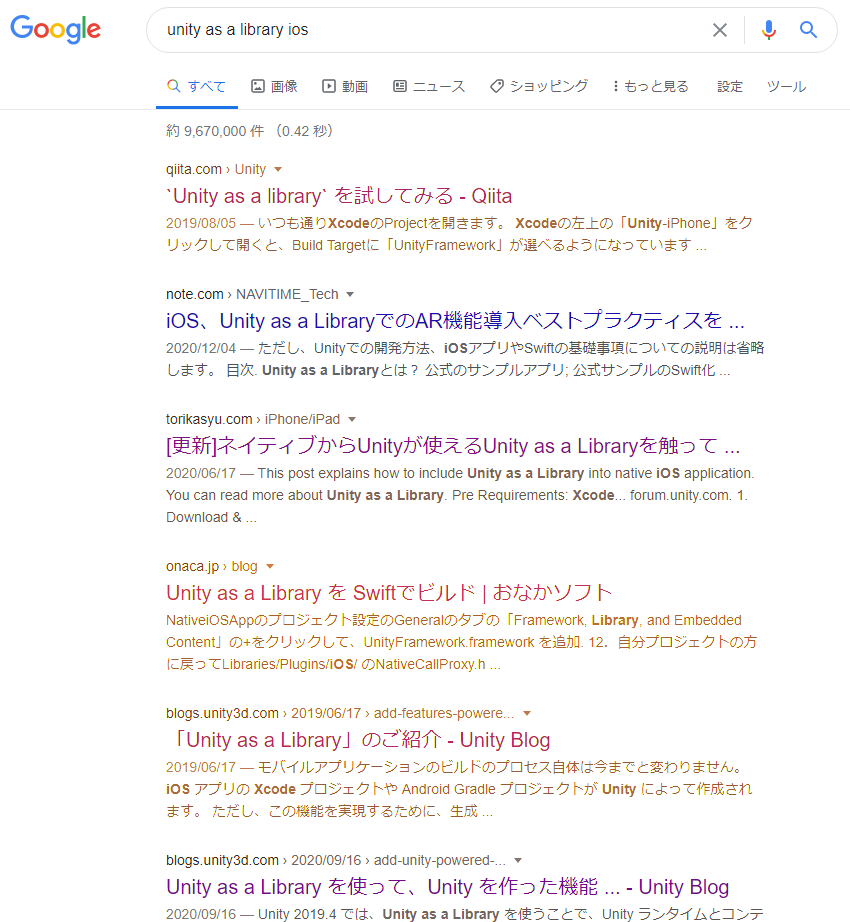
\includegraphics[width=60mm]{images/ink2.png}}
    \end{center}
    \caption{インクの劣化をイメージした視覚化2}
    \label{fig:ver-ink2}
  \end{minipage}
\end{figure}

\ref{subsec:ver-col-cor}と同様に、情報の鮮度に応じて文字の色が焦げ茶色に近づくようにしたのが図\ref{fig:ver-ink1}である。

また、背景色の白に薄まるように変化を加えたのが図\ref{fig:ver-ink2}である。

図\ref{fig:ver-ink1}に関しては、視覚化による変化が目立っておらずユーザに情報の鮮度を認識させるという目的が果たせていない。

図\ref{fig:ver-ink2}は、古い印象を与えることには成功しているが、古いか新しいかの二択に捉えられやすいと思われる。

どちらの場合も段階的な変化を認識しやすい視覚化の方法とは言えない。

\section{文字の消失による変化}
\label{sec:ver-character}

文字の一部、または全体を欠落させたり存在感を薄めることで鮮度を視覚化する方法を検証する。

\subsection{透明化}
\label{subsec:ver-chr-trp}

実世界のモノが時間経過によって消失していくさまをイメージして、各項目の不透明度を変更することで鮮度の視覚化を行った。

\begin{figure}[htbp]
  \begin{center}
    \fbox{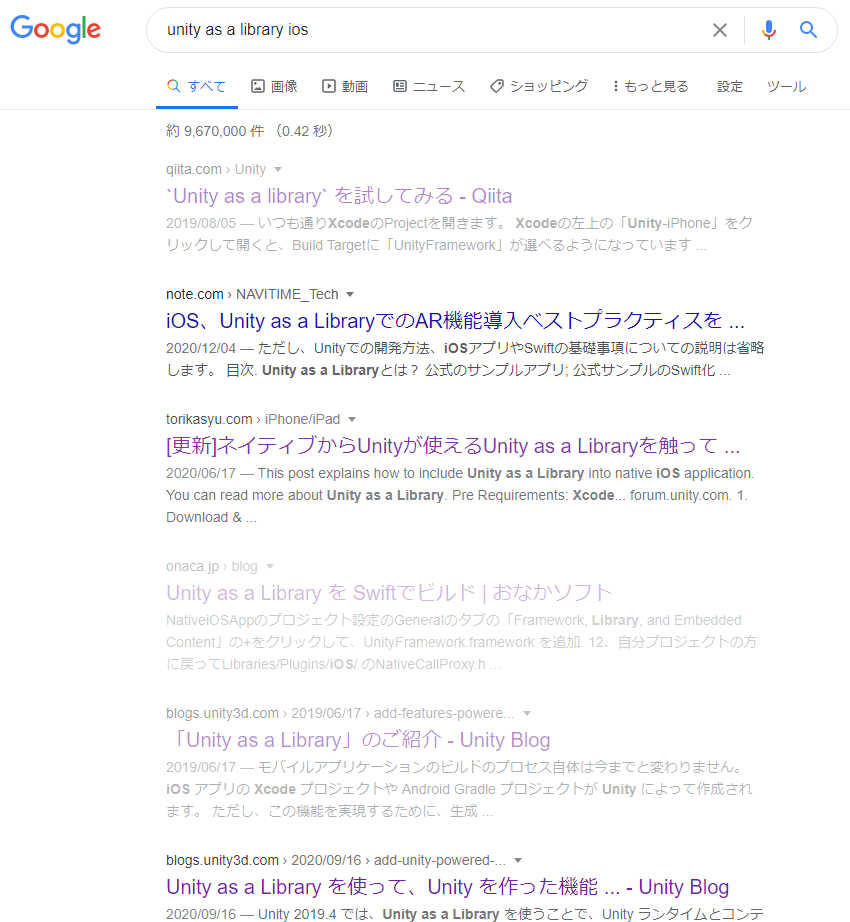
\includegraphics[width=60mm]{images/transparence.png}}
  \end{center}
  \caption{不透明度を変更した視覚化}
  \label{fig:ver-transparence}
\end{figure}

図\ref{fig:ver-transparence}は、各情報ごとに古いければ古いほど不透明度が下がっていくように視覚化を行ったものである。

元の検索画面に対して微小な変更のみを加えているため、不自然な点が少ない。また、段階的な変化が認識しやすく時間経過を簡単に見て取れる。

しかし薄いもの(不透明度が低いもの)が古いという結びつけが弱いため、鮮度を表しているという認識を与えられるか疑問がある。

\subsection{滲む}
\label{subsec:ver-chr-bld}

紙にインクをたらしたときにインクが滲んでいくイメージを参考に、鮮度を視覚化した。

\begin{figure}[htbp]
  \begin{center}
    \fbox{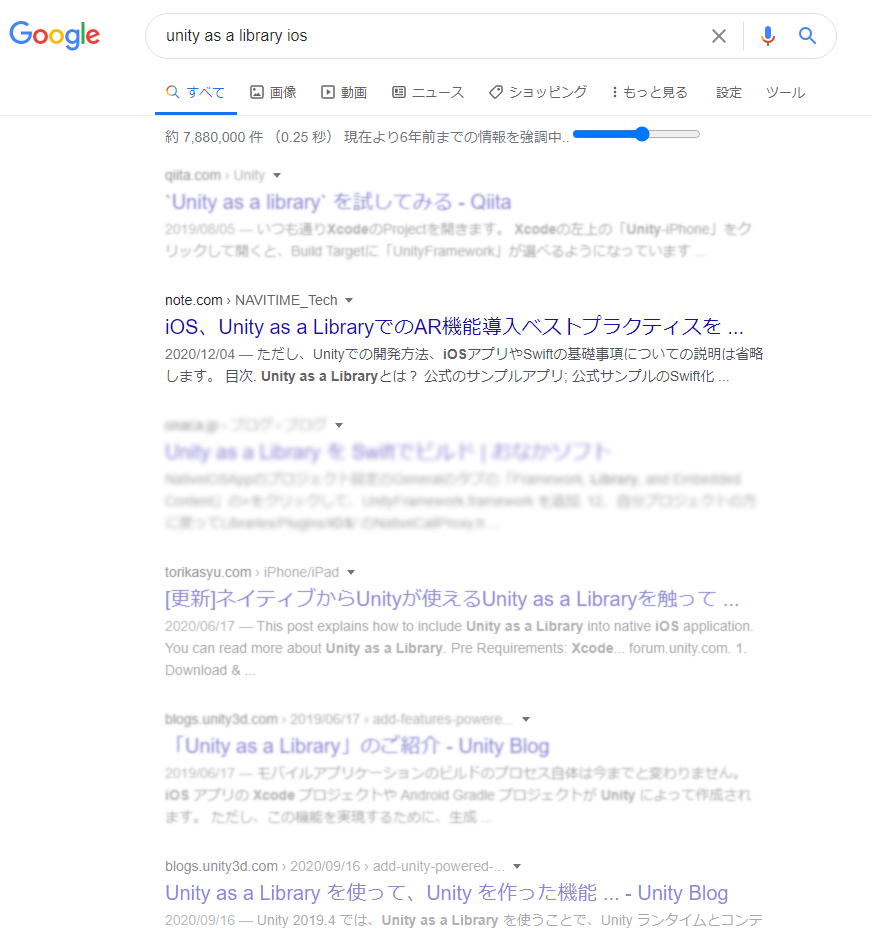
\includegraphics[width=60mm]{images/bleeding.png}}
  \end{center}
  \caption{インクの滲みをイメージした視覚化}
  \label{fig:ver-bleeding}
\end{figure}

\ref{subsec:ver-chr-trp}と同様の基準で、文字が滲むように変更を加えたのが図\ref{fig:ver-bleeding}である。

透明化のように元の背景とよくなじみ、段階的な変化が感じやすい。加えて、古いものを読ませないという効果も期待できる。

しかしながら、やはり滲んでいるから古い情報だという結びつけは弱いのではないだろうか。

\subsection{虫食い}
\label{subsec:ver-chr-wh}

古い書物などは紙自体の経年劣化の他にシミなどの虫による欠落が見られる。そういった劣化の仕方を参考に鮮度を視覚化した。

\begin{figure}[htbp]
  \begin{minipage}{0.5\hsize}
    \begin{center}
      \fbox{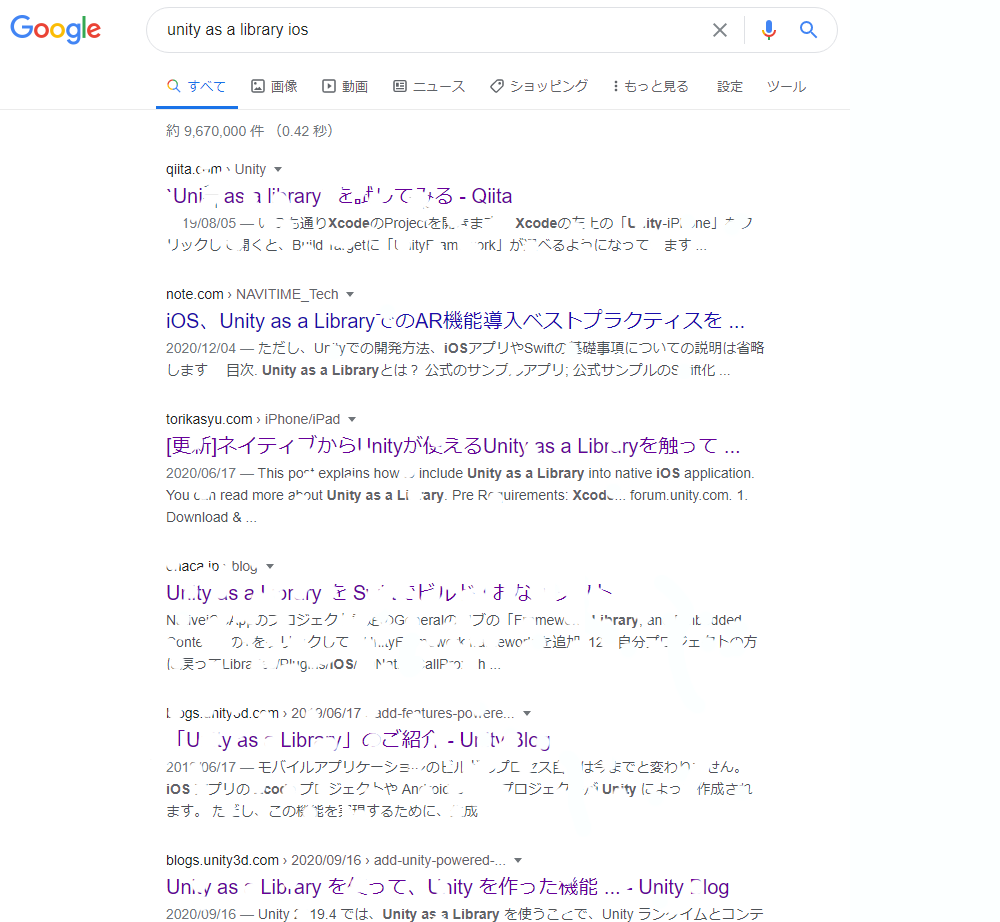
\includegraphics[width=60mm]{images/wormhole1.png}}
    \end{center}
    \caption{虫食いをイメージした視覚化1}
    \label{fig:ver-wormhole1}
  \end{minipage}
  \begin{minipage}{0.5\hsize}
    \begin{center}
      \fbox{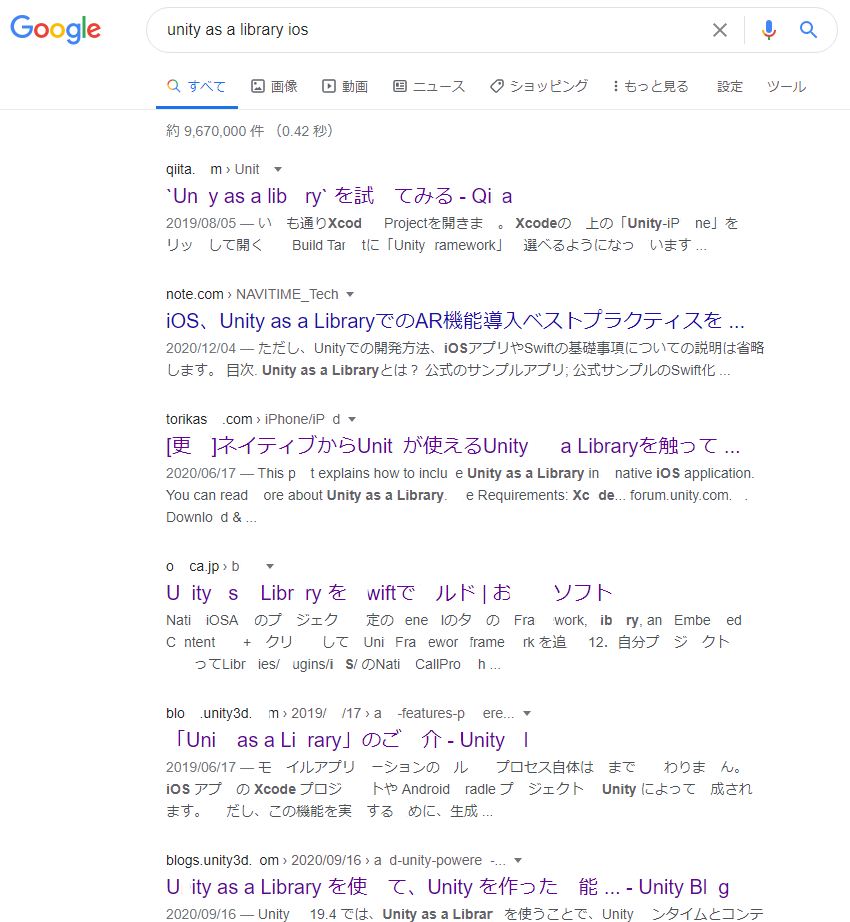
\includegraphics[width=60mm]{images/wormhole2.png}}
    \end{center}
    \caption{虫食いをイメージした視覚化2}
    \label{fig:ver-wormhole2}
  \end{minipage}
\end{figure}

図\ref{fig:ver-wormhole1}は実際に虫に食われた紙をイメージして、古いものがより欠損するように視覚化を行ったものである。

そして図\ref{fig:ver-wormhole2}は文章の虫食いをイメージして、古ければ古いほど多くの文字が欠落するように視覚化を行ったものである。

どちらも情報の鮮度に応じた変化の程度の差を設けるのが難しいが、古いものを読ませない効果は十分にあるだろう。

しかし、ある程度の文字が欠損していても何となくで読めてしまう部分があり、\ref{subsec:ver-col-ink}の視覚化と同様、段階的な変化ではなく読めるか読めないかの二分された認識になった。

\section{フォントによる変化}
\label{sec:ver-font}

使用されるフォントを変更することで鮮度を視覚化する方法を検証する。

\subsection{書体}
\label{subsec:ver-fnt-stl}

時代が進むごとに文字の書体も変わってきた\footnote{5分で学ぶフォントの歴史500年|時代背景とタイポグラフィ, https://note.com/smartcamp-design/n/n2740a3b72be9}。

古い情報は古そうだと感じられる書体を、新しい情報は新しそうだと感じられる書体を用いて記述することで情報の鮮度を視覚化した。

\begin{figure}[htbp]
  \begin{center}
    \fbox{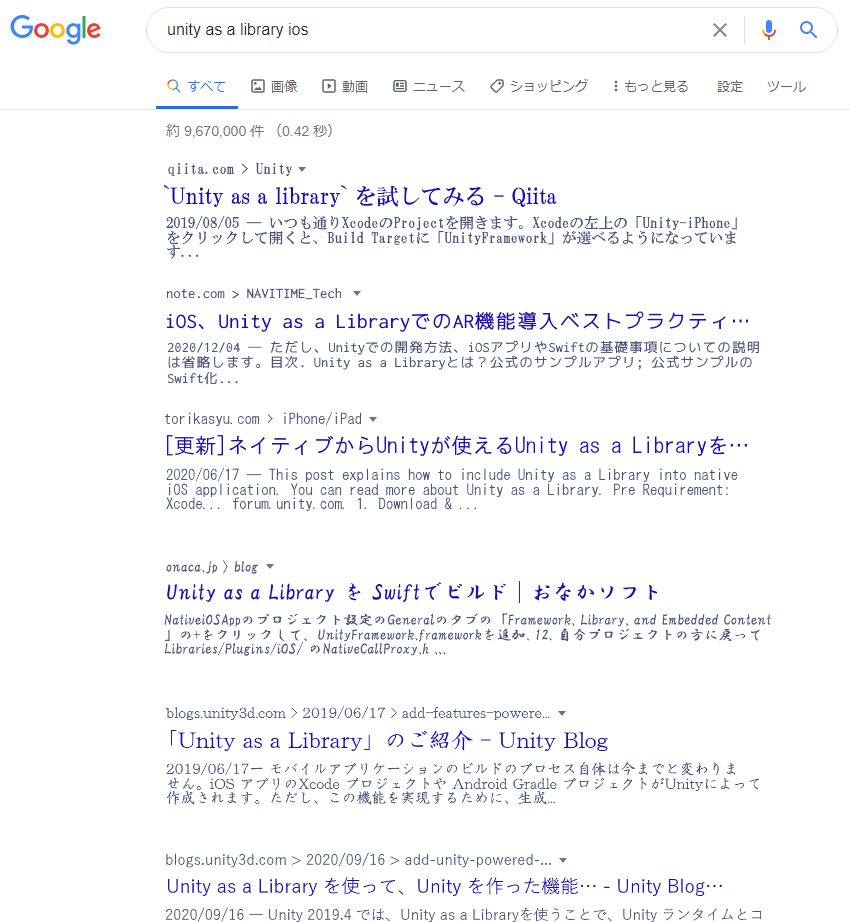
\includegraphics[width=60mm]{images/font-style.png}}
  \end{center}
  \caption{書体の変化による視覚化}
  \label{fig:ver-style}
\end{figure}

図\ref{fig:ver-style}は各情報ごとにWindowsに標準で搭載されているフォントを用いて、鮮度を視覚化したものである。

検証して分かったことだが、フォントの選定が難しく、人によって感じる印象が違うため鮮度を表すものとしては適さないと考えられる。

\subsection{ドット文字}
\label{subsec:ver-fnt-dot}

古い電子機器の画面ではピクセル数の関係からドット文字が使用されていたり、古さを演出するために意図的にドット文字を使うこともある。

そこで粒度の違うドット文字を用いて情報の鮮度を視覚化した。

\begin{figure}[htbp]
  \begin{center}
    \fbox{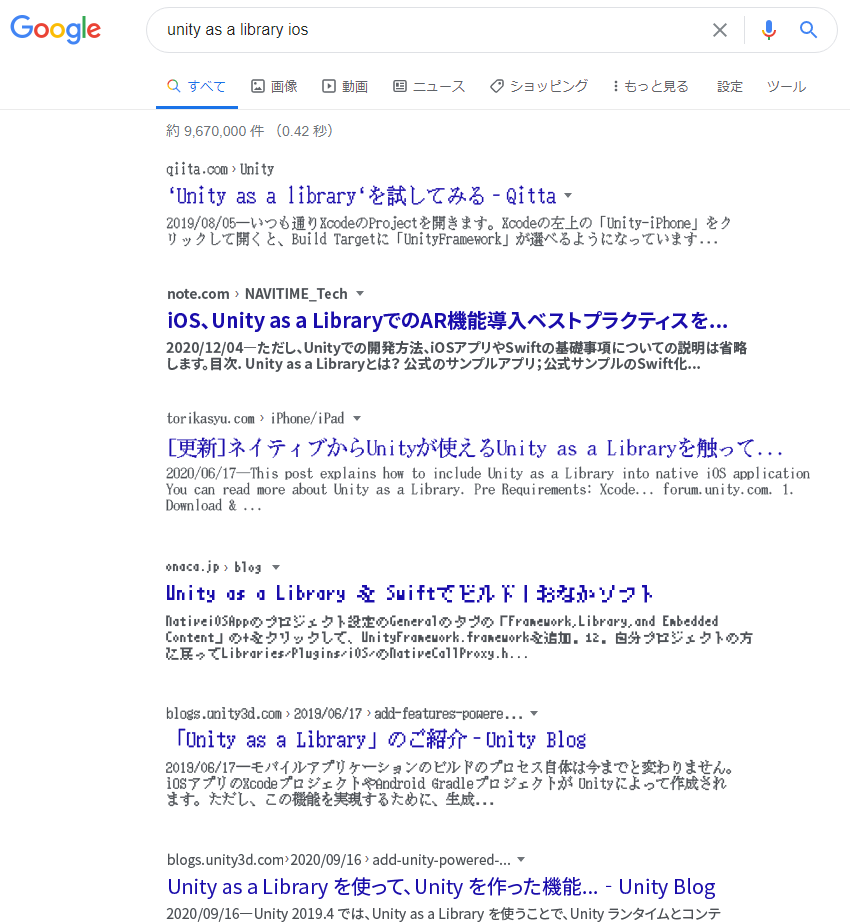
\includegraphics[width=60mm]{images/font-dot.png}}
  \end{center}
  \caption{ドット文字の粒度の変化による視覚化}
  \label{fig:ver-dot}
\end{figure}

古ければ古いほど粒度の荒いドット文字を使って表現したのが図\ref{fig:ver-dot}である。

予測では鮮度の段階ごとの変化を感じやすいと思われたが、古い印象よりも各サイトごとの特色だという印象の方が強かった。

これは各ドット文字がそれぞれ特徴的で、段階的な変化を感じさせなかったためだと推測される。

\section{その他の変化}
\label{sec:ver-other}

以上までに分類されない変化を用いて鮮度を視覚化する方法を検証する。

\subsection{テロメア}
\label{subsec:ver-oth-tlm}

Scrapboxというサービス\footnote{\url{https://scrapbox.io/}}内で用いられている、更新時刻を視覚化する機能\footnote{\url{https://scrapbox.io/shokai/%E3%83%86%E3%83%AD%E3%83%A1%E3%82%A2}}を参考に情報の鮮度の視覚化を行った。

\begin{figure}[htbp]
  \begin{center}
    \fbox{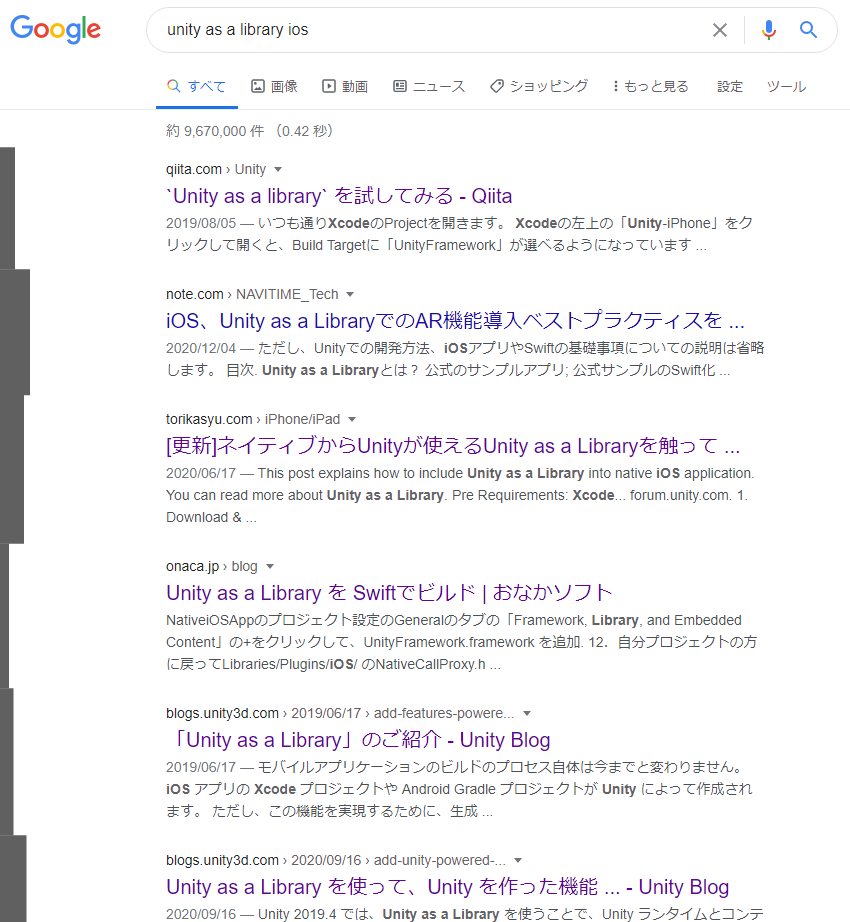
\includegraphics[width=60mm]{images/telomere.png}}
  \end{center}
  \caption{テロメアによる視覚化}
  \label{fig:ver-telomere}
\end{figure}

図\ref{fig:ver-telomere}は画面左端にテロメアを適用したものである。

各情報の鮮度ごとの段階的な変化が分かりやすく、それぞれの程度の差も直感的に感じられる。

しかし、同サービスを利用した経験がないユーザにはこれが情報の鮮度を表したものだと認識しにくいのではと推測される。

  % 本文2
\chapter{鮮度の視覚化の実装}
\label{chap:implementation}

本章では、第\ref{chap:verification}章で検証した鮮度の表現方法を参考に、実際にブラウザで動作する拡張機能の実装について述べる。

  % 本文3
\chapter{議論}
\label{chap:discussion}

本章では、第\ref{chap:implementation}章で開発した拡張機能を実際に運用した結果と評価について述べ、それを踏まえて議論を行う。

\newpage

\section{筆者の運用}

筆者は本拡張機能を開発段階から3か月程度利用した。利用している中で感じたのは、Web 上には古い情報が大量に存在しているということである。

新しい情報と古い情報がすべて均一に並べられていたという事実を今まで意識してこなかったことが痛感できた。また、全体を一覧した際にどの情報の鮮度がいいのかをすぐに識別可能で、新しい情報が欲しい際などにすぐに見つけることができた。

\section{第三者の意見}

研究会のメンバーの一人に本システムを実際に利用してもらい、フィードバックをもらった。

古いものが見えにくくなる点については、検索する分野によってはその分野の情報全体が古い場合があり、外見的な劣化が全体におよんでしまうという意見があった。

しかし同時に、情報の鮮度が視覚化されることによって通常の Web 検索に比べて、見ている情報の古さを意識できるようになったと評価された。

\section{関連研究}

廃れるリンク\cite{dyinglink}は Web 上のリンクに対して「モノが廃れる」メタファを適用することで、リンクの鮮度を一目で判断させること目的としたシステムである。

本研究との違いは、適用するメタファの選定や鮮度の算出部分の他に、こちらはブラウザにおける検索結果一覧に絞ったものという点である。

特に鮮度の算出に関して、廃れるリンクではプロキシサーバーを利用した大規模のものになっているが、本研究ではローカルの Chrome 拡張のみで動作することができるため、導入も容易である。

\section{今後の展望}

検証、実装および運用を経て、二つの問題点が浮かび上がった。

\begin{itemize}
  \item 情報の分野ごとに全体の鮮度の平均が違う
  \item 正確な情報の鮮度を取得できないことがある
\end{itemize}

それぞれに関しての考察と展望を以下に述べる。

\subsubsection{分野ごとの鮮度}

情報の分野によっては全体の鮮度が古い場合が存在する。例えば、既に更新が止まっている昔の技術を利用しようと検索をした場合、出てくる情報はいずれも古くなるのが必然である。

あるいは情報がすくない場合、一覧されるの情報の鮮度もバラツキが生まれ、外見的な劣化を加えることで本来よりも知りたい情報にたどり着きにくくなってしまう恐れがある。

そこでユーザが自由に、鮮度の算出を行う際の閾値を設定できるようにし、かつ、検索ワードごとの閾値のおススメを表示できるようにすれば、本システムの利点を残したまま、検索精度をあげることができる可能性がある。

\subsubsection{正確な鮮度の取得}

本システムでは検索結果一覧に並んでいる Google Chrome が表示している各項目の更新日時を参考にして鮮度を算出している。

しかし、Chrome の表示する更新日時は正確ではないこともあり、場合によっては表示されていないこともある。本システムでは更新日時が表示されていない情報に関しては、最も古いものとして扱っている。

他に更新日時を知る方法として該当リンク先のページで document.lastModified を実行して、時刻データを入手する方法がある。しかしこの方法はページの仕様によっては、コードを実行した時の時刻が返ってきてしまう。

筆者が調べた限りでは、現状全てのサイトごとの正確な鮮度を知る方法はなく、各サイトごとの更新者が申請する以外にない。それらを集めたデータベースなどを作る方法が考えられるが現実的とは言い難い。

この問題は今後の課題としたい。
  % 本文4
\chapter{関連研究}
\label{chap:survey}

本章では,Web 検索や Web ページにおける情報の視覚化の中で関連がある研究を本研究との対比を交えながら紹介する.

\newpage

\subsubsection{廃れるリンク}

廃れるリンク\cite{dyinglink}は Web 上のリンクに対して「モノが廃れる」メタファを適用することで,リンクの鮮度を一目で判断させること目的としたシステムである.

本研究との違いは,適用するメタファの選定や鮮度の算出部分の他に,こちらはブラウザにおける検索結果一覧に絞ったものという点である.特に鮮度の算出に関して,廃れるリンクではプロキシサーバーを利用した大規模のものになっているが,本研究ではローカルの Chrome 拡張のみで動作することができるため,導入も容易である.

\subsubsection{テロメア}

テロメア\cite{telomere}は Scrapbox\footnote{\url{https://scrapbox.io/}} の機能で,行の更新時刻を視覚化する.行の更新時刻が一目でわかり,鮮度を対数関数で計算することで,長いスパンでも新旧が視覚化できる.

編集可能なデータに関してはこの視覚化が有効だが,本研究のシステムで適用した場合(図\ref{fig:ver-telomere}),鮮度を表すものだと認識し難い.

\begin{figure}[htbp]
  \begin{center}
    \fbox{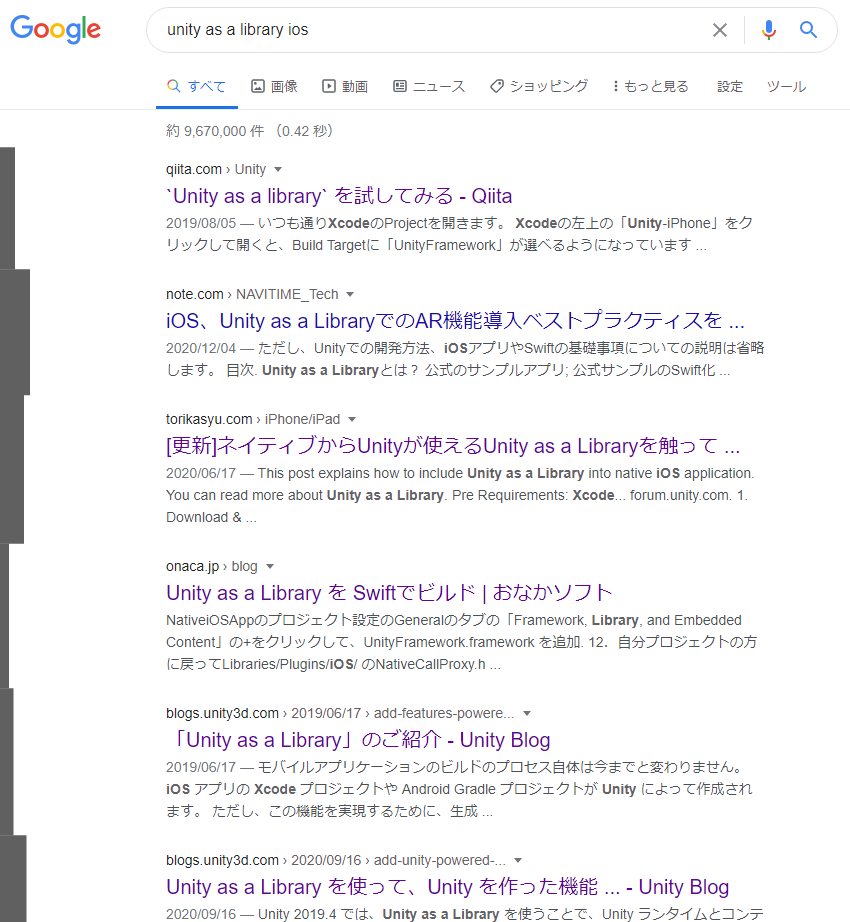
\includegraphics[width=60mm]{images/telomere.png}}
  \end{center}
  \caption{テロメアによる視覚化}
  \label{fig:ver-telomere}
\end{figure}

\subsubsection{分類動作を取り入れたウェブ検索支援システムの構築}

森\cite{classify}らは,検索結果の内容を吟味させる方法として,一覧画面でユーザに結果の分類行動を要求している.本研究の直感的という部分に該当しないが,ユーザに各情報の鮮度を吟味させる手法として効果が期待できる.

また,再検索を行う際に原因分析をユーザが行うアプローチは,本研究に鮮度以外の尺度を設ける手段として活用できる.
  % 本文5
\chapter{結論}
\label{chap:conclusion}

本章では,本研究で得られた成果について述べる.

\newpage

本研究では,ブラウザにおける検索結果一覧画面を拡張することで情報の鮮度を視覚化するシステムの設計および実装を行った.

本システムにより,ユーザが今までのブラウジングでは注意してこなかった情報の鮮度を直感的に認識させることが可能となり,情報の鮮度に注意を払うように促す効果も期待できた.

運用を通して,我々が普段閲覧している Web 上には古い情報が多く存在していることを改めて認識させられた.今までのブラウザが Web 検索結果一覧画面で,情報の鮮度を意識させていなかったのは大きな問題である.

また,時間経過のみを参考にした鮮度の割り出しでは,足りない側面もあった.情報の更新内容や前回更新からの経過時間など,鮮度の算出に検討すべきパラメーターがいくつも見つかった.

情報の鮮度の表現方法や,鮮度の算出方法に残る課題もこれからの開発で解決していきたい.
  % 本文6

\begin{acknowledgment}

本研究を進めるにあたり、ご指導いただきました増井井俊之先生に深く感謝いたします。

同じく、研究アイデアに対して多大なアドバイスをくださった左治木隆成氏をはじめとする増井研究会に所属している方々にも感謝の意を表します。ありがとうございました。

\end{acknowledgment}
  % 謝辞.要独自コマンド,include先参照のこと

\begin{bib}[100]
% BibTeXを使う場合
\bibliography{main}

%\begin{thebibliography}{#1}
%
%  \bibitem{参照用名称}
%    著者名: 
%    \newblock 文献名,
%    \newblock 書誌情報,出版年.
%
% \bibitem{hoge09}
%   ほげ山太郎,ほげ山次郎:
%   \newblock ほげほげ理論のHCI分野への応用,
%   \newblock ほげほげ学会論文誌,Vol.31,No.3,pp.194-201,2009.
% 
% \bibitem{hoge08}
%   Taro Hogeyama, Jiro Hogeyama:
%   \newblock The Theory of Hoge,
%   \newblock {\it The Proceedings of The Hoge Society}, 2008.
%	
%\end{thebibliography}

\end{bib}
  % 参考文献.要独自コマンド,include先参照のこと
\appendix
% \chapter{付録の例}

付録を無理矢理出力させるため,てきとうなことを書く.

\section{ほげ}

コマンドは本文と一緒.

\subsection{ふー}

本文と一緒.

\section{ほげほげ}

本文と一緒.

\subsection{ふーふー}

本文と一緒.
    % 付録

\end{document}
